\chapter{Datasets utilizados}

\section{High-Resolution Fundus (HRF)}
Consiste en 18 pares de imágenes de la misma retina, capturadas con una cámara Canon CR-1 con un campo de visión de 45°. Cada par contiene una imagen de mala calidad y una imagen de mejor calidad, representando situaciones en las que la exploración tuvo que repetirse debido a deficiencias en la adquisición.

Las imágenes de baja calidad presentan problemas como desenfoque global o localizado, generalmente causado por un enfoque incorrecto de la cámara. Ambas imágenes de cada par comparten aproximadamente el mismo campo visual, aunque pueden presentar pequeños desplazamientos debido a movimientos involuntarios del ojo durante la captura. El nombre de cada archivo corresponde con el número identificador de la retina y la etiqueta de calidad \parencites{koehler2013automatic}.

\begin{center}
	\begin{figure}[H]
		\centering
		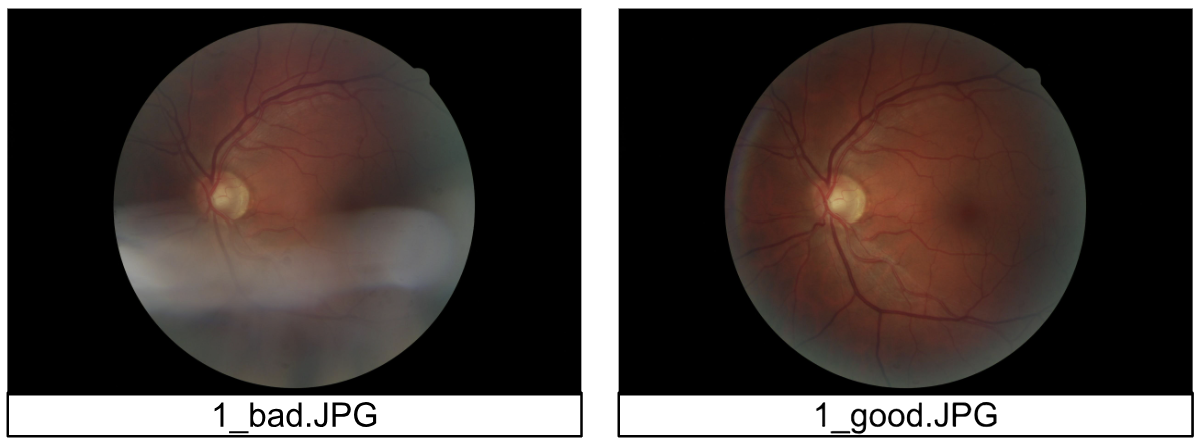
\includegraphics[scale=0.80]{doc_images/HRF.png}
		\caption{Ejemplo de imágenes de fondo de ojo del dataset HRF.} 
		\label{fig:HRF}
	\end{figure}
\end{center}

\section{DDR}
Contiene 13,673 imágenes en color de fondo de ojo obtenidas entre 2016 y 2018 de 9,598 pacientes en 147 hospitales de 23 provincias de China. La recopilación siguió criterios de distribución uniforme en cuanto a edad, género y procedencia geográfica de los pacientes, asegurando la diversidad en el conjunto de datos.

Las imágenes fueron capturadas con 42 tipos de cámaras de fondo de ojo con un campo de visión de 45°, incluyendo modelos como Topcon D7000, Topcon TRC NW48, Nikon D5200 y Canon CR-2.

Cada imagen fue etiquetada por siete especialistas según la Clasificación Internacional de Retinopatía Diabética, asignándolas a una de seis categorías: No DR, DR no proliferativa leve, DR no proliferativa moderada, DR no proliferativa severa, DR proliferativa, No calificable (imágenes con más del 70\% de desenfoque y sin lesiones claramente visibles).

La categorización de las imágenes siguió un proceso de votación entre los especialistas. En caso de desacuerdo, se consultaron oftalmólogos con más de 30 años de experiencia para la decisión final.

\begin{center}
	\begin{figure}[H]
		\centering
		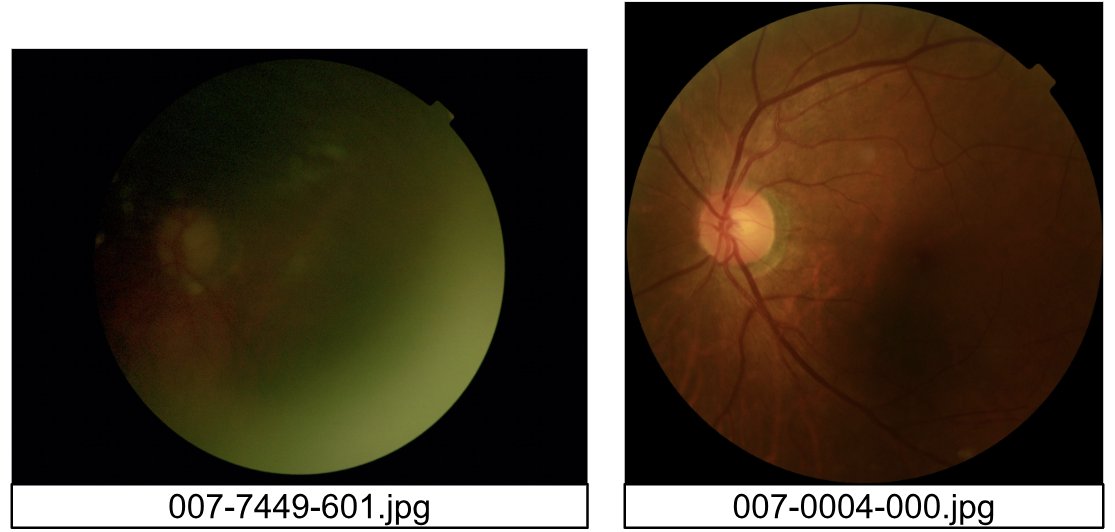
\includegraphics[scale=0.80]{doc_images/DDR.png}
		\caption{Ejemplo de imágenes de fondo de ojo del dataset DDR, (izquierda: No clasificable, derecha: No DR).} 
		\label{fig:DDR}
	\end{figure}
\end{center}

\section{Deep Diabetic Retinopathy Image Dataset (DeepDRiD)}
El DeepDRiD es un conjunto de datos desarrollado para la competencia Diabetic Retinopathy: Segmentation and Grading Challenge, organizada en conjunto con el Simposio Internacional de IEEE sobre Imágenes Biomédicas (ISBI 2020). Su propósito es evaluar métodos de clasificación automática de la retinopatía diabética (DR) y la calidad de imágenes de fondo de ojo.

El dataset está compuesto por imágenes obtenidas de pacientes incluidos en diferentes estudios en Shanghai, como el Shanghai Diabetic Complication Screening Project, el Nicheng Diabetes Screening Project y el Nation-wide Screening for Complications of Diabetes. Además, se incorporaron imágenes adquiridas en la clínica de oftalmología del Sixth People’s Hospital of Shanghai Jiao Tong University. De los miles de exámenes disponibles, se seleccionaron aleatoriamente 2.000 imágenes de fondo de ojo regulares correspondientes a 500 pacientes. Cada paciente tiene cuatro imágenes de fondo de ojo, con dos imágenes por ojo: una centrada en la mácula y otra en el disco óptico.

Las imágenes se separaron 60\% (1.200 imágenes) para entrenamiento, 20\% (400 imágenes) para validación y 20\% (400 imágenes) para evaluación. Las imágenes de este dataset están etiquetadas en un archivo CSV, donde la variable Overall quality indica la calidad de la imagen: 0 para imágenes de mala calidad y 1 para imágenes de buena calidad (Liu et al., 2022). En este trabajo, solo se utilizan los conjuntos de entrenamiento y validación, ya que para el conjunto de evaluación no están disponibles las etiquetas. Las 1.600 imágenes se utilizarán exclusivamente para la fase de prueba, sin formar parte del entrenamiento del modelo.

\begin{center}
	\begin{figure}[H]
		\centering
		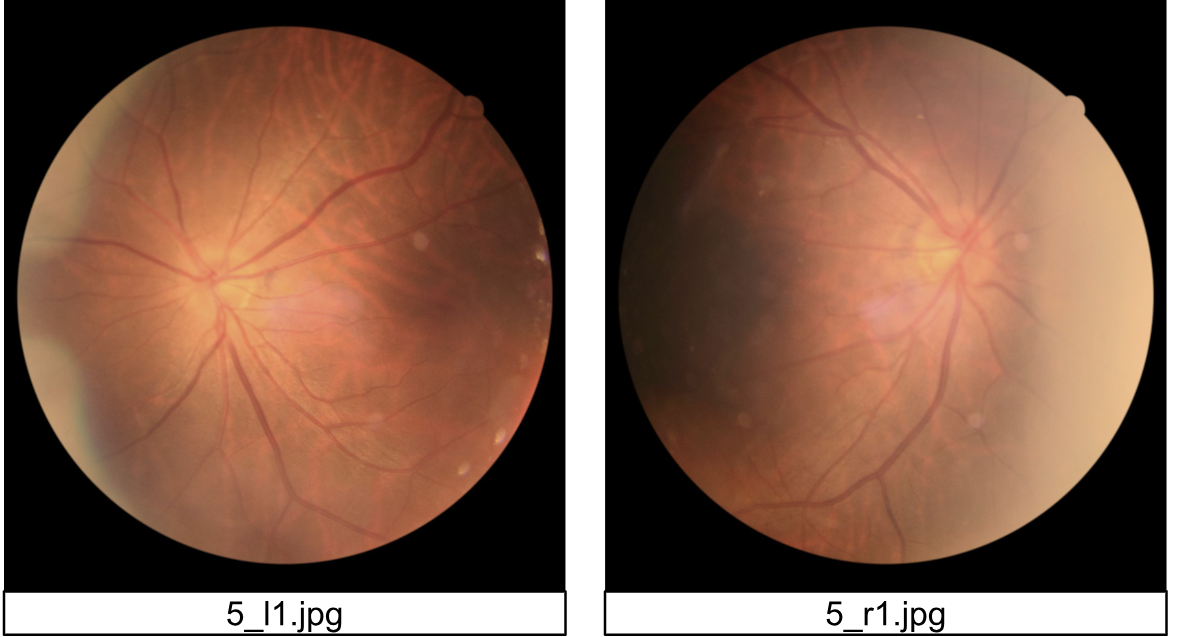
\includegraphics[scale=0.80]{doc_images/DeepDRiD.png}
		\caption{Ejemplo de imágenes de fondo de ojo del dataset DeepDRiD, (izquierda: buena calidad, derecha: mala calidad).} 
		\label{fig:DeepDRiD}
	\end{figure}
\end{center}

\section{Kaggle DR Dataset}
Este conjunto de datos contiene imágenes de retina proporcionadas por EyePACS\footnote{EyePACS: es una red de telemedicina que proporciona acceso a exámenes de retina para la detección de retinopatía diabética y otras enfermedades oculares. \url{https://eyepacs.com/}} para la competencia organizada por Kaggle\footnote{\url{https://www.kaggle.com/c/diabetic-retinopathy-detection/overview}} y la California Healthcare Foundation, con el objetivo de desarrollar modelos de detección de retinopatía diabética. Contiene miles de imágenes capturadas con diferentes modelos y tipos de cámaras, con variaciones en términos de iluminación, enfoque y calidad en general. Sin embargo, este conjunto de datos no incluye etiquetas explícitas de calidad de imagen.

Para obtener etiquetas de calidad, se utilizó la versión etiquetada por profesionales propuesta por \parencites{zhou2018deep}, denominada Kaggle DR Image Quality Dataset, en la que las imágenes fueron clasificadas en dos categorías: 0 para imágenes de mala calidad y 1 para imágenes de buena calidad. Este conjunto de datos está dividido en 35,126 imágenes para entrenamiento, 10,906 para validación y 42,670 para evaluación. Las etiquetas de calidad están almacenadas en archivos CSV, con un archivo separado para cada partición (entrenamiento, validación y evaluación). Cada CSV contiene el nombre de la imagen y su respectiva etiqueta en el campo quality.


\begin{center}
	\begin{figure}[H]
		\centering
		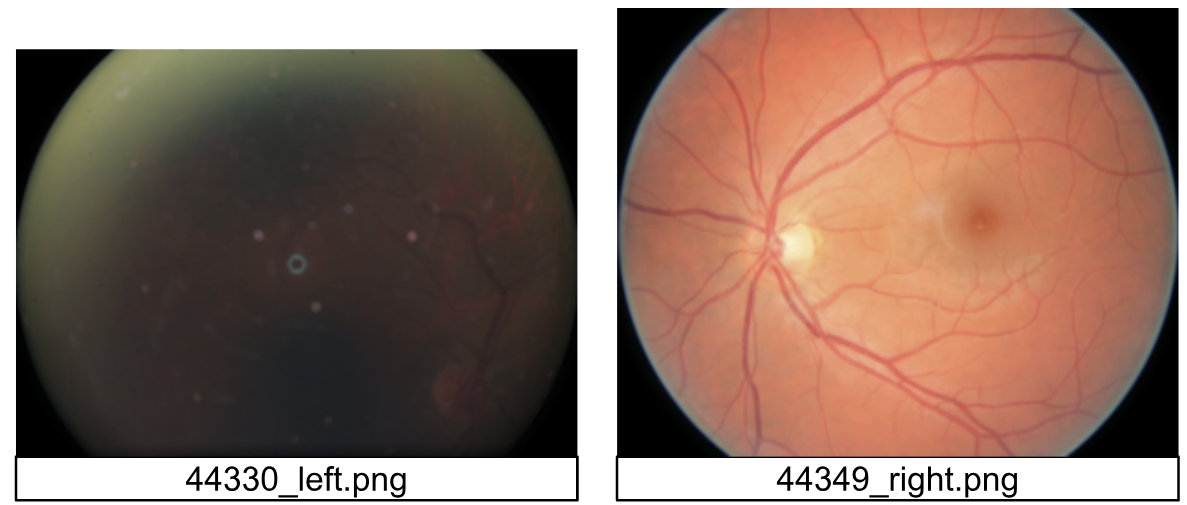
\includegraphics[scale=0.80]{doc_images/Kaggle.png}
		\caption{Ejemplo de imágenes de fondo de ojo del dataset Kaggel, (izquierda: mala calidad, derecha: buena calidad).} 
		\label{fig:Kaggle}
	\end{figure}
\end{center}

El cuadro \ref{tab:dataset_count} presenta un resumen con la cantidad de imágenes utilizadas en los subconjuntos de entrenamiento, validación y test.

\begin{table*}[h]
	\centering
	\renewcommand{\arraystretch}{1.5}
	\resizebox{\textwidth}{!}{
	\begin{tabular}{ |c|c|c|c|c|c|c|c|c|c|  }
		\hline
		\multirow{2}{*}{\textbf{Dataset}}&\multicolumn{3}{|c|}{\textbf{Train}} &\multicolumn{3}{|c|}{\textbf{Validation}} &\multicolumn{3}{|c|}{\textbf{Test}} \\
		\cline{2-10}
		 & \textbf{Buena} & \textbf{Mala} & \textbf{Total} & \textbf{Buena} & \textbf{Mala} & \textbf{Total} & \textbf{Buena} & \textbf{Mala} & \textbf{Total} \\
		\hline
		HRF & 9 & 9 & 18 & 6 & 6 & 12 & 3 & 3 & 6 \\
		\hline
		DDR & 6,260 & 575 & 6,835 & 2,503 & 230 & 2,733 & 3,759 & 346 & 4,105 \\
		\hline
		DeepDRiD & - & - & - & - & - & - & 758 & 842 & 1,600 \\
		\hline
		Kaggle & 33,840 & 1,285 & 35,125 & 10,680 & 226 & 10,906 & 41,797 & 873 & 42,670 \\
		\hline
		\hline
		Total & 40,109 & 1,869 & 41,978 & 13,189 & 462 & 13,651 & 46,317 & 2,064 & 48,381 \\
		\hline
	\end{tabular}
	}
	\caption{Distribución de imágenes por dataset, clase y partición.}
	\label{tab:dataset_count}
\end{table*}